\documentclass[12pt,english]{scrartcl}
\usepackage{amsmath,booktabs}
\usepackage{amssymb}
\usepackage{amsthm}
\usepackage[a4paper,
            left=25mm,
            right=25mm,
            top=25mm,
            bottom=25mm,
            headsep=10mm]{geometry}
\usepackage[utf8]{inputenc}
\usepackage{mathtools}
\usepackage{tikz,graphicx}
\usepackage{pgfplots}
\usepackage{wrapfig}
\usepackage{hyperref}
\usepackage[capitalize]{cleveref}
\usepackage{mdframed}

% Backwards compatibility for pgfplots
\pgfplotsset{compat=1.17}

% Style hyperlinks
\hypersetup{
    colorlinks=true,
    linkcolor=blue,
    filecolor=magenta,
    urlcolor=cyan,
}
\urlstyle{same}

% Path to images
\graphicspath{{./img/}}

% Math macros
\newcommand{\R}{\mathbb{R}}

% Theorem styles
\theoremstyle{definition}
\newtheorem{definition}{Definition}[section]
\newtheorem{theorem}{Theorem}[section]
\theoremstyle{remark}
\newtheorem{observation}{Observation}[section]
\newtheorem*{remark}{Remark}

% Tweak display settings
\renewcommand*{\titlepagestyle}{empty}
\renewcommand{\thesection}{\arabic{section}}
\renewcommand{\footnotesize}{\fontsize{9pt}{11pt}}
\deffootnote[1em]{1em}{1em}{\textsuperscript{\makebox[1em][l]{\thefootnotemark}}}

% Normal heading elements
\title{\vspace{-1.5cm}
\includegraphics[scale=1.50]{1F4DA.pdf} Math Review} % Emoji hack ;)
\subtitle{DA Learning \& Development}
\author{Ravi Dayabhai}

\begin{document}
\maketitle

This is a brief primer (or refresher, depending on your background) of the core
concepts from calculus that will help ease the transition from ``Pebble World'' (and the
discrete distributions that we've encountered in our tour of the Distribution
Zoo so far) to the next exhibit: the \emph{continuous distributions}. You've
likely encountered a few of these in your mathematical career already (e.g.,
the Normal).  Adding these distributions to our toolkits is essential to make
sense of bedrock ideas in statistics (e.g., the Central Limit Theorem), but
before we get ahead of ourselves, let's make sure we feel comfortable with the
basic underpinnings that enable us to reckon with these new and exotic
distributions.

\section{Functions}%
\label{sec:functions}

We've already touched on sets (see Lesson 2 material in our
\href{https://github.flexport.io/rdayabhai/da_prob_stat/tree/master/Lesson_2}{repo}),
so we'll start by taking a closer look at \textbf{functions}.

\begin{definition}[Function] A function is a relation that associates each
    element $x$ of a set $X$, called the \textit{domain} of the function, to a
    single element $y$ of another set $Y$ (possibly the same set), the
    \textit{codomain} of the function. We can write this as
    \[
        f \colon X \mapsto Y
    .\]
\end{definition}

Intuitively, a function is a deterministic rule that ``maps'' an element from
one set to an element in another set. Another interpretation is that functions
are ``machines,'' taking inputs and producing outputs. (It's easy to see
why these objects are central to computer science as well.) Importantly,
different $x$'s can map to the same $y$, but each $x$ only maps to one $y$
(e.g., the ``vertical line test'' from grade school).

\begin{remark} We should take care to distinguish $f$ from $f(x)$. The former
    is the function itself, the rule; the latter is a number for each number
    $x$. As in programming, a function (treated as an object) is not the same
    thing as what the function returns when called with a particular set of
    arguments.  \end{remark}

Certain table relations can be thought of functions: ``one-to-one'' or
``many-to-one'' are examples of this. A ``one-to-many'' table relation violates
the definition of a function, even if its \textit{inverse} is a valid function.
In this way, we don't need to restrict ourselves to numbers. In fact, we've
already seen functions in the context of probability when we defined random
variables\footnote{\textbf{random variable} $\coloneqq$ a function that maps
the sample space to real numbers or vectors}.

\subsection{Injective, Bijective, and Surjective Functions}%
\label{sub:injective_bijective_and_surjective_functions}

Let $f \colon A \mapsto B$. We can describe or characterize this function by
the relationship between its domain ($\forall a \in A$) and codomain
($\forall b \in B$).

\begin{definition}[Injective Function] A function is said to be
    \textita{injective} or ``one-to-one`` if  $f(a_{1}) \neq f(a_{2})$ whenever
    $a_{1} \neq a_{2}$.  Any two distinct inputs to the function get mapped to
    two distinct outputs.  Said another way: for every $b$ there can be at most
    one $a$ that maps to it.
\end{definition}

\begin{definition}[Surjective Function] A function is said to be
    \textita{surjective} or ``onto'' if  $\forall b \in B , \exists a \in A,
    f(a) = b$. Said another way: every $b$ has a corresponding $a$, but the
    converse may not necessarily be true.
\end{definition}

\begin{definition}[Bijective Function] A function is said to be bijective or
    ``one-to-one correspondence'' if it is both injective and surjective.
\end{definition}

A key distinction to make is between ``one-to-one'' and ``one-to-one
correspondence'': the latter describes a function as being both injective and
surjective, whereas the former describes it as being injective only. The terminology
may seem clunky at first, but with
\href{https://brilliant.org/wiki/bijection-injection-and-surjection/}{a little
practice}, it makes talking about functions much easier.

\subsection{Increasing and Decreasing Functions}%
\label{sub:increasing_and_decreasing_functions}

Using the same function $f$ from above, we can fashion two straightforward
definitions for increasing and decreasing functions:

\begin{definition}[Increasing Function] If $a_{1} \leq a_{2} \implies f(a_{1})
    \leq f(a_{2})$, then $f$ is said to be \textit{increasing} over $[a_{1},
    a_{2}]$.
\end{definition}

\begin{definition}[Decreasing Function] If $a_{1} \leq a_{2} \implies f(a_{1})
    \geq f(a_{2})$, then $f$ is said to be \textit{decreasing} over $[a_{1},
    a_{2}]$.
\end{definition}

Note that these definitions allow for flat regions. \textit{Strictly}
increasing or decreasing restricts these definitions a bit more (read: replace
the $\leq, \geq$ with $<, >$, respectively in the definitions above). Another
word to describe increasing or decreasing functions is \textit{monotone} (e.g.,
letting $f(x) = x^{3}$,  $f$ is \textit{monotonically} increasing).

\begin{remark}
    Any strictly monotone function is one-to-one (i.e., injective).
\end{remark}

\subsection{Even and Odd Functions}%
\label{sub:even_and_odd_functions}

Let $f \colon \R \mapsto \R$. This simply means the function $f$ maps
\textit{real} numbers to \textit{real} numbers in one dimension. (Without
digressing too much, a function $g \colon \R^{2} \mapsto \R^{3}$ means $g$ is a
\textit{vector}-valued function from two dimensions to three.)

\begin{definition}[Even Function] If, $\forall x$ in the domain of $f$, $f(x) =
    f(-x)$, then $f$ is an \textit{even} function.
\end{definition}

\begin{definition}[Odd Function] If, $\forall x$ in the domain of $f$, $-f(x) =
    f(-x)$, then $f$ is an \textit{odd} function.
\end{definition}

\begin{remark}
    A function that exhibits neither property is neither even nor odd.
\end{remark}

Even and odd functions exhibit symmetries: even functions can be reflected
across the $y$-axis (in $\R^{2}$) and odd functions have rotational
symmetry around the origin. We can leverage these properties when we need to
take integrals. Even functions have the property that, for any $a$,

\[
    \int_{-a}^{a} f(x) \mathop{dx} = 2 \int_{0}^{a} f(x) \mathop{dx}
,\] and odd functions have the property that, for any $a$, \[
\int_{-a}^{a} f(x) \mathop{dx} = 0
.\]

\noindent(\textbf{Hint:} Draw a picture to see why this is true.)

\section{Calculus}%
\label{sec:calculus}

In ``Pebble World'', we dealt with \textit{countably} finite (or infinite)
supports\footnote{
    \textbf{support} $\coloneqq$ all values a random variable can
    take; if $X$ is a discrete random variable, then the finite or countably
    infinite set of values x such that $P(X = x) > 0$ is called the support of $X$
}, which made it easy to relate pebbles to numbers. Now, we're
leaving the comfort of counting with integers behind and venturing into the
\textit{uncountable}.

\subsection{Real Numbers}%
\label{sub:real_numbers}

Earlier, we talked about \textbf{real} numbers, but let's remind ourselves of
what they are.

\begin{figure}[ht]
    \centering
    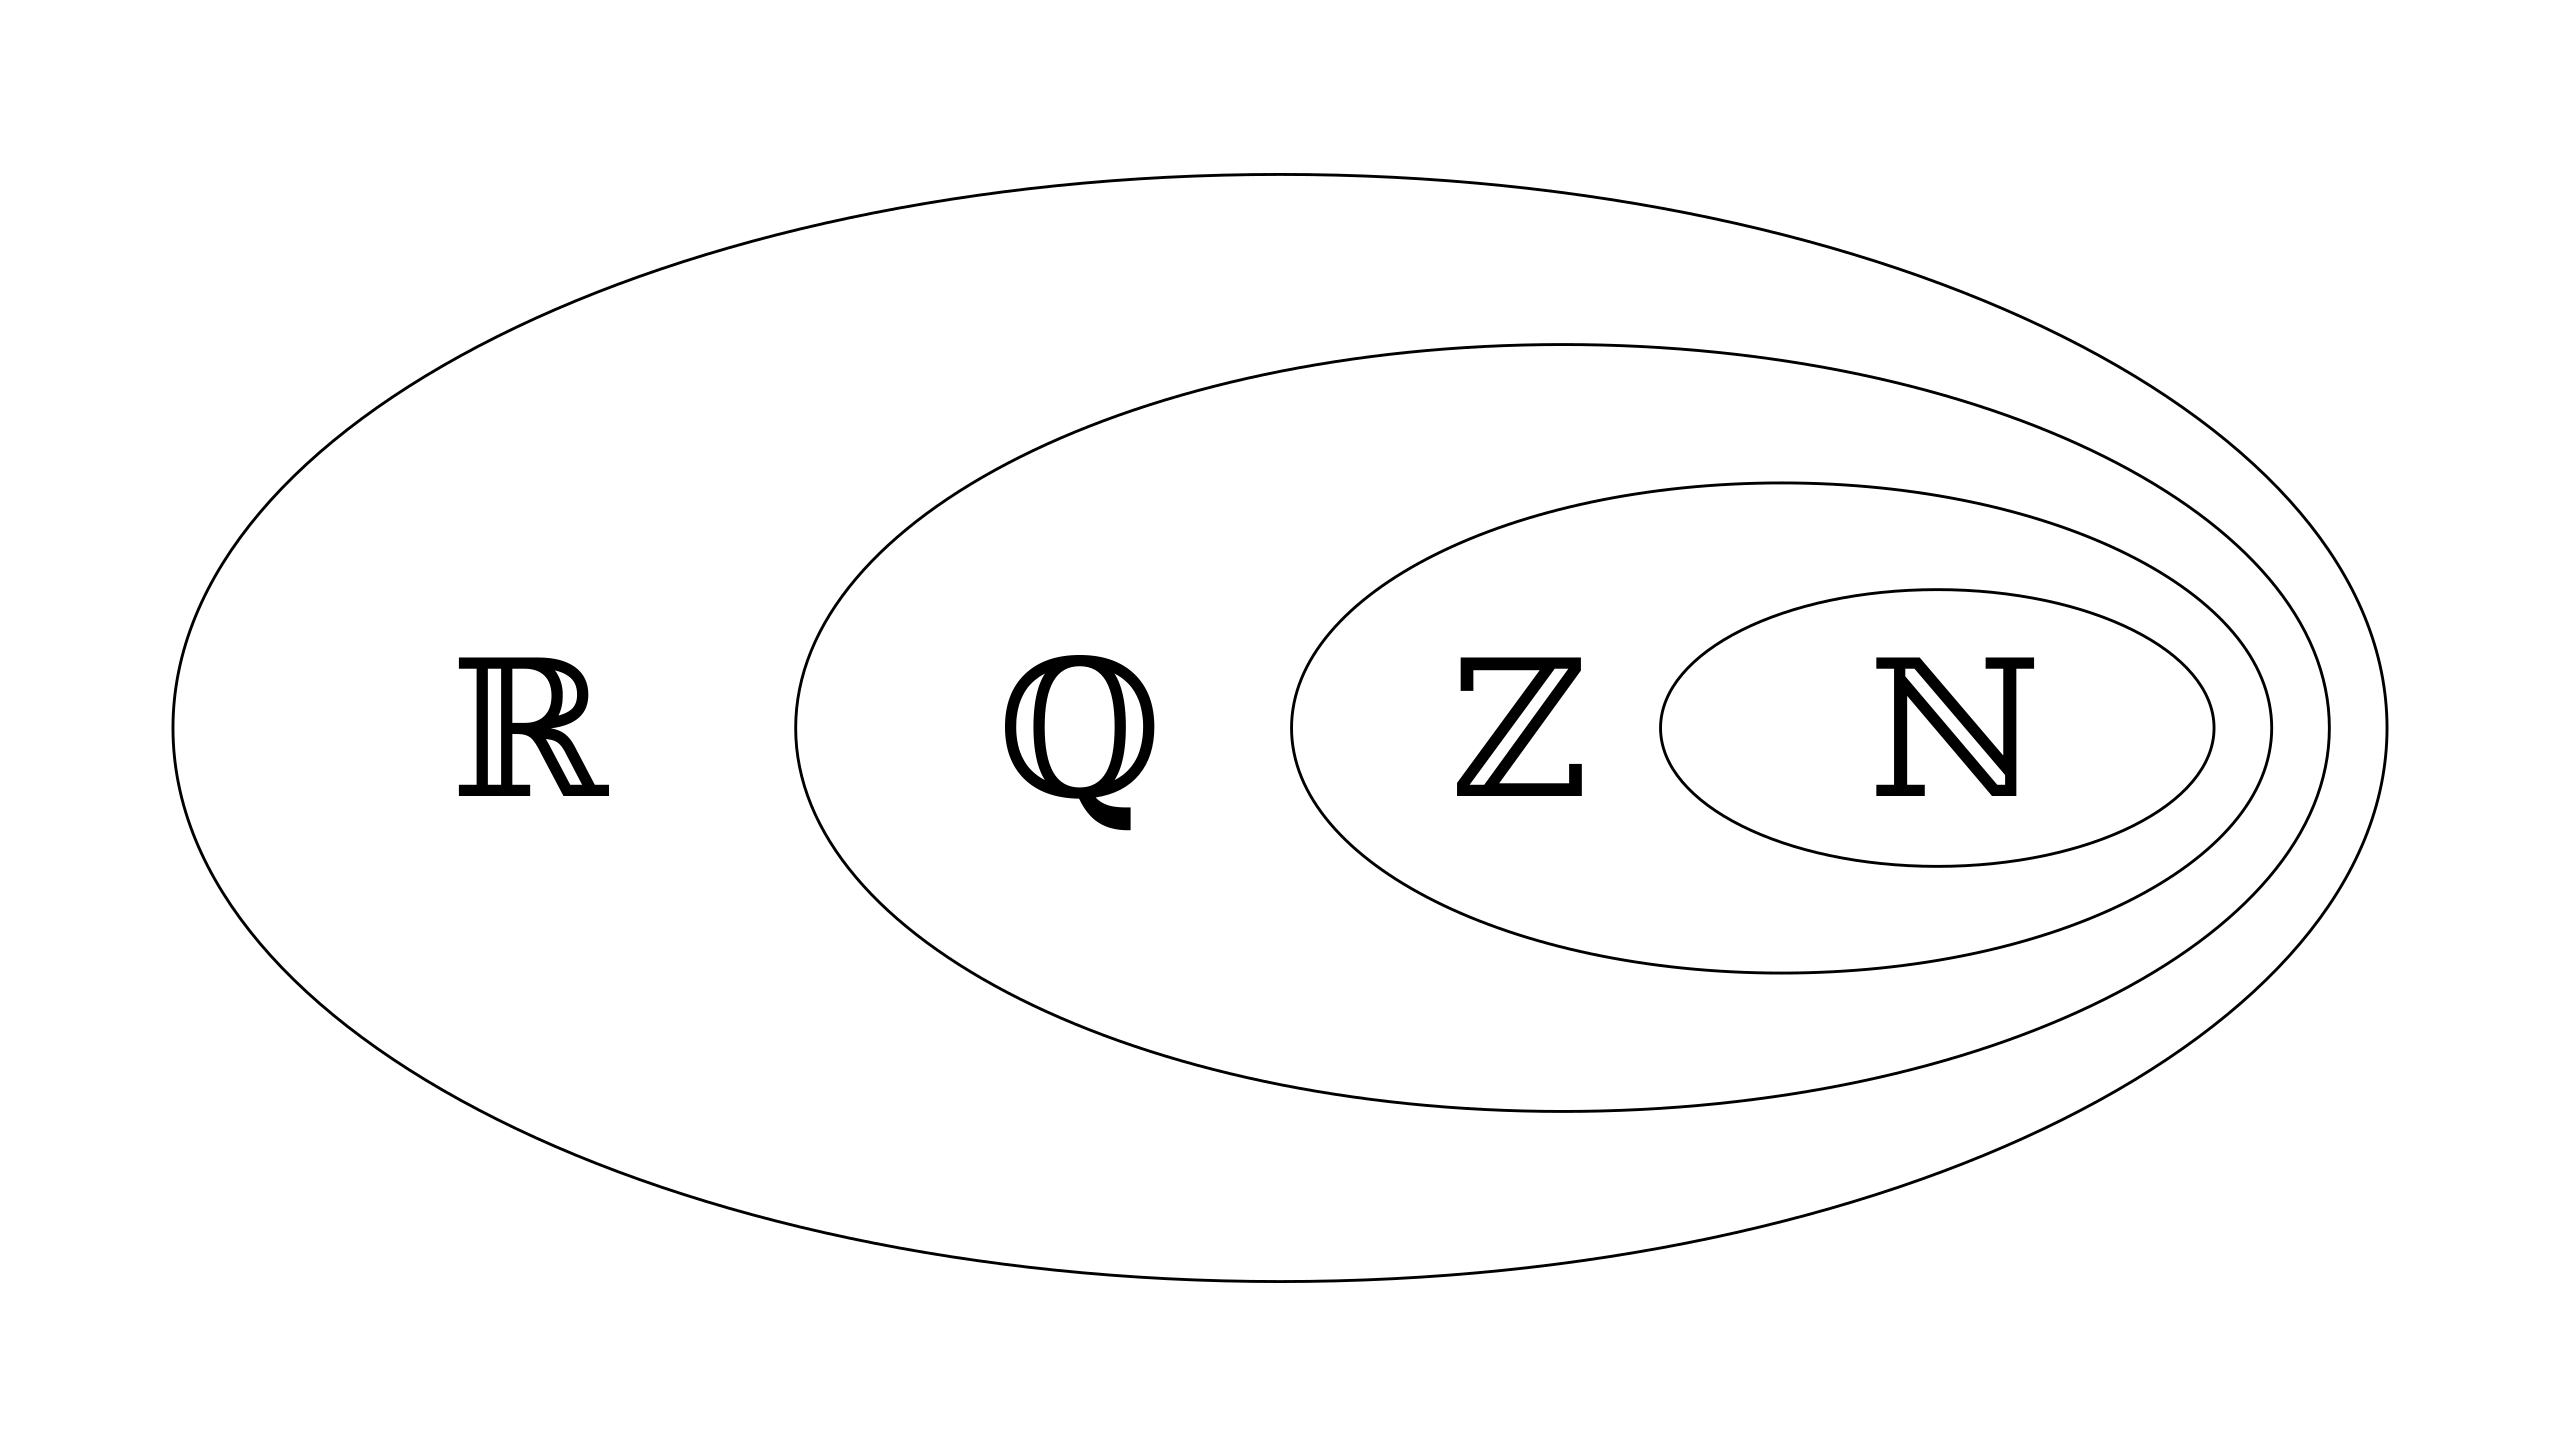
\includegraphics[width=0.5\linewidth]{number-systems}
    \caption{$\mathbb{Q}$ are the \textit{rationals}; $\mathbb{R}$ are the \textit{reals} }
    \label{fig:number-systems}
\end{figure}

\begin{definition}[Rational Numbers] A rational number is a number such as
    $\frac{-3}{7}$ that can be expressed as the quotient or fraction
    $\frac{p}{q}$ of two integers, a numerator $p$ and a non-zero denominator
    $q$.
\end{definition}

\begin{definition}[Irrational Numbers] An irrational number is a number that
    cannot be expressed as the quotient or fraction $\frac{p}{q}$ of two
    integers, a numerator $p$ and a non-zero denominator $q$. Examples include
    $\pi$, $e$, $\sqrt[3]{2}$, $\sqrt{2}$, and a bunch of others, to say the
    least (in fact, probability helps to intuit that
    \href{https://math.stackexchange.com/a/474496/300506}{there are ``more''
    irrationals than rationals}).
\end{definition}

\begin{definition}[Real Numbers] The set of real numbers is the union of the rational
    and irrational numbers. Real numbers can be thought of as points on an
    infinitely long line (called the ``number line'' or ``real line''), where the points
    corresponding to integers are equally-spaced.
\end{definition}

There are infinitely many integers, and they are \textit{countable}. There are
infinitely many real numbers, but they are \textit{uncountable}. In fact, the
``smoothness'' of a continuous function over a given interval arises because
the function is defined for all, infinite reals in that interval (read: no
``gaps'' anywhere). The main idea to transplant to your mental model for
probability should be that we no longer can rely on counting or ``weighing''
individual ``pebbles''!

\subsection{Limits}%
\label{sub:limits}

Let's now return to what it means to ``take the limit'' of a function at a
certain point, $a$, and how this notion allows us to make the logical leaps
necessary to work on a continuum in probability.

\begin{definition}[Limits]
    The limit of $f(x)$ as $x$ approaches $a$ is a
    number $L$, written
    \begin{equation*}
        \lim_{x \to a} f(x) = L
    \end{equation*}
    if the value of $f(x)$ is as close as one wishes to $L$ for
    all $x$ sufficiently close, but not equal to $a$.
    \label{def:limits}
\end{definition}

The best case scenario is when $f(a) = L$ (this means $f$ is
\textit{continuous} at $a$ when combined with \cref{def:limits}), but this need not be
necessarily true (e.g., removable discontinuities) for the limit to exist.
Luckily, for our purposes, we won't worry about discontinuities (in general)
because the distributions we will be studying are called \textit{continuous}
distributions for a reason!

The notion of a limit is, however, important when we think about ``adding up''
(think: integrating) under a \textit{probability density function} (PDF) whose
domain is over $(-\infty, \infty)$ -- the area under a PDF must be $1$ in the
same way the total mass of pebbles in ``Pebble World'' sums to $1$. This is
discussed more in \cref{sub:differentiation_integration} below.

\subsection{Differentiation \& Integration}%
\label{sub:differentiation_integration}

We won't burden ourselves with a rigorous treatment of these topics, but we
should call out the big ideas. First, a useful theorem to segue us from
\cref{sub:limits}:

\begin{theorem}
    If a function $f(x)$ is differentiable in some interval, then it is
    also continuous in that interval. The converse may not be true.
\end{theorem}

If you can take the derivative of a function over some interval then you know
the function is continuous over that interval. Later, we'll see this means we're
permitted to differentiate a continuous random variable's CDF to yield its PDF.

\begin{figure}[ht]
    \centering
    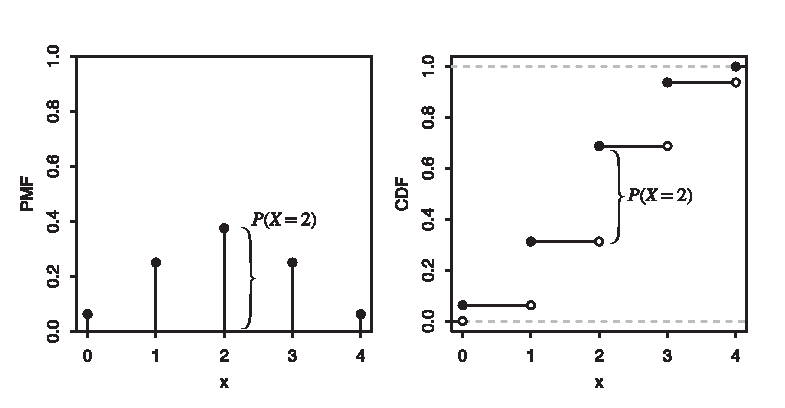
\includegraphics[width=0.75\linewidth]{pmf_cdf}
    \caption{Even in the discrete setting, the PMF ``feels'' like the derivative of the CDF.}
    \label{fig:pmf_cdf}
\end{figure}

Remember, we can fully describe a discrete distribution with either the CDF or
the PMF (or the parameters and class of distribution, e.g., $\text{Bin}(n,
p)$). Discrete CDFs have jumps, and these jumps correspond to values of the
PMF, as seen in \cref{fig:pmf_cdf}.  We could also start with the PMF and
construct the CDF. This sensation (of going back and forth between two related
functions) is the most fundamental idea of calculus -- so fundamental, in fact,
that it's called the \textbf{Fundamental Theorem of Calculus} (FTC).  The two
variants of the FTC demonstrate how $F$ and $f$ characterize each other.

\begin{theorem}[Fundamental Theorem of Calculus: Part 1 (FTC 1)]
    \label{thm:ftc_1}
    If $f$ is continuous and $F'(x) = f(x)$, then \[
        \int_{a}^{b} f(x) \mathop{dx} = F(b) - F(a)
    .\]
\end{theorem}

\begin{theorem}[Fundamental Theorem of Calculus: Part 2 (FTC 2)] If $f$ is continuous and
    $G(x) = \int_{a}^{x} f(t) \mathop{dt}$, then $G'(x) = f(x)$. Note that
    $G(x) = F(x) + C$, where $C$ is a constant. The exact value for $C$ depends
    on the choice of $a$. This can be confirmed by \cref{thm:ftc_1}.
\end{theorem}

Stare at this for a while if some time has passed since you last acquainted
yourself with calculus -- it's not that bad, I promise! In short, these two
theorems establish the following, key insight:

\begin{mdframed}[leftmargin=30, rightmargin=30]
\textbf{Integration and differentiation are inverse operations}, in the same
way addition and subtraction are inverse operations of each other.  \[
    \color{blue}{x^2} \color{black}\xrightarrow{\displaystyle\int}
    \color{red}{\frac{x^3}{3}  \;(\,+\,C\,)}
    \color{black}\xrightarrow{\displaystyle\frac{d}{dx}} \color{blue}{x^2}\]
\end{mdframed}


Another way to reason about integration ($\int$) is that it is the continuous
analog of summation ($\sum$). We can think of the [signed] area under the graph of
$f(x)$ as approximating the sum of all of the rectangles formed by height
$f(x)$ and width $\Delta x$, which is just some small, non-zero length that evenly
divides $(a,b)$. This approximation gets better as we let $\Delta x \to 0$ because
this means we're now generating more (albeit thinner) rectangles, per
\cref{fig:riemann_sum}. (Grant Sanderson does a much better job of
\href{https://www.youtube.com/watch?v=rfG8ce4nNh0}{making this idea come to
life} than I can here.)

\begin{figure}[ht]
    % \centering
        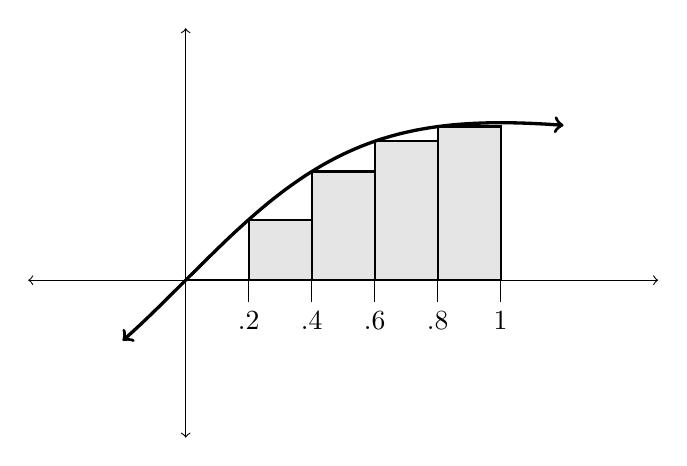
\begin{tikzpicture}[scale=4]
            \draw[<->] (-.5,0) -- (1.5,0);
            \draw[<->] (0,-.5) -- (0,.8);
            \foreach \x in {0,.2,...,.8}
                \draw[thick, fill=gray!20] (\x,0) -- (\x,{\x/(1+\x*\x)}) -- (\x+.2,{\x/(1+\x*\x)}) -- (\x+.2,0) -- cycle;
            \draw[very thick, <->, domain=-.2:1.2, smooth, variable=\x] plot ({\x},{\x/(1+\x*\x)});
            \foreach \x in {.2,.4,.6,.8,1}
                \draw (\x,2pt) -- (\x,-2pt) node[below] {\x};
        \end{tikzpicture}
        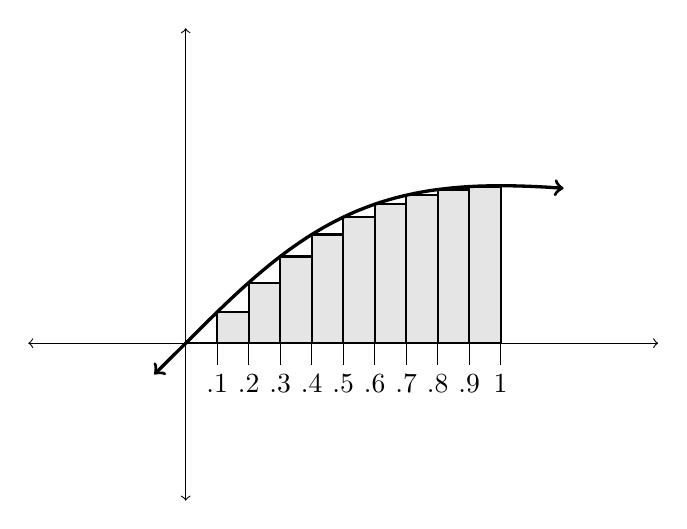
\begin{tikzpicture}[scale=4]
            \draw[<->] (-.5,0) -- (1.5,0);
            \draw[<->] (0,-.5) -- (0,1);
            \foreach \x in {0,.1,...,1}
                \draw[thick, fill=gray!20] (\x,0) -- (\x,{\x/(1+\x*\x)}) -- (\x+.1,{\x/(1+\x*\x)}) -- (\x+.1,0) -- cycle;
            \draw[very thick, <->, domain=-.1:1.2, smooth, variable=\x] plot ({\x},{\x/(1+\x*\x)});
            \foreach \x in {.1,.2,.3,.4,.5,.6,.7,.8,.9,1}
                \draw (\x,2pt) -- (\x,-2pt) node[below] {\x};
        \end{tikzpicture}
    \caption{Smaller choices of $\Delta x$ $\implies$ more rectangles $\implies$ better approximation of the area under the curve}
    \label{fig:riemann_sum}
\end{figure}

\begin{remark}[Notation] Leibniz's notation (e.g., $\frac{dy}{dx}$) is a great
    reminder of what's going on: $f(x)$, the derivative of $F(x)$, tells us how
    much a ``little nudge'' to $x$ ($\Delta x$) affects $F(x)$. Making this
    nudge smaller and smaller (read: $\Delta x \to 0$ over all $x$'s) is
    precisely the idea captured by the notation -- the \textit{limit} as the
    size of the nudges approaches $0$ is $dx$ and the effect on $F(x)$ of these
    nudges (in the limit) is what we call $dF(x)$ (or $dy$ when $y=F(x)$). The
    ratio of these two quantities in the limit (i.e., $\frac{d}{dx}F(x)$) is what
    the derivative is!
\end{remark}


But what does summing up the areas of ever-thinner rectangles (i.e., ``areas
under curves'') have to do with the differences of two quantities, namely,
$F(b)-F(a)$? (See \cref{thm:ftc_1}.) It's pretty remarkable that we can
describe a certain area under $f(x)$ just by looking at two points on the graph
of $F$!

First, consider what information is encoded by $f$: per the definitions above,
\[
F'(x) = \frac{d}{dx}F(x) = f(x)
.\]

So, if integrating $f$ from $a$ to $b$ is just doing some sort of ``fancy
sum'', and $f$ describes vanishingly tiny nudges to $F$ (due to vanishingly
tiny nudges to $x$, i.e., $dx$), then it stands to reason that integrating
``brings together'' all of the accumulated nudges of $F$ from $a$ to $b$ \ldots
but this is precisely what $F(b)-F(a)$ describes!}

We can apply this logic to the two primary functions that govern continuous random
variables, namely, the CDF $F_{X}(x)$ and PDF $f_{X}(x)$ (for a continuous
random variable $X$).  Again, the notation suggests what our intuition leads us
to believe: integrating the PDF yields the CDF and differentiating the CDF
yields the PDF.  We'll have more to say about this when we visit these
distributions in the Distribution Zoo, but \cref{fig:pdf_cdf} below illustrates this
notion.

\pagebreak

\begin{figure}[ht]
    \centering
    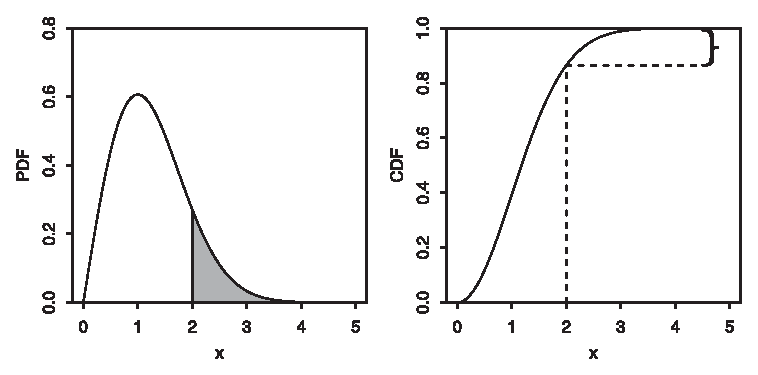
\includegraphics[width=0.75\linewidth]{pdf_cdf}
    \caption{The area of the shaded region (left) under the PDF is the same thing as the difference between the CDF for the corresponding values of $x$ (right).}
    \label{fig:pdf_cdf}
\end{figure}

\subsection{Taylor Series}%
\label{sub:taylor_series}

Taylor series help us to approximate a function about a point using
polynomials.

\begin{definition}[Taylor Series] Let $f(x)$ be a real-valued function that is infinitely
    differentiable at $x = x_0$. The Taylor series expansion for the function
    $f(x)$ centered around the point $x = x_0$ is given by
    \nopagebreak[4]
    \[
    \sum_{n=0}^{\infty}f^{(n)}(x_0)\frac{(x - x_0)^{n}}{n!}
    .\]

    Note that $f^{(n)}(x_0)$ represents the $n^\text{th}$ derivative of $f(x)$
    at $x = x_0$. If we choose $x_{0} = 0$, we get a special case of this
    approximation method, which is called the \textbf{Maclaurin series}.
\end{definition}

This is an extremely powerful approximation technique that leverages the fact
that polynomials are relatively easy to deal with (e.g., taking repeated
derivatives means applying the power rule over and over again) and can be
applied to functions that would be hard to directly compute. The reason we get
better approximations as we add more terms is because the added terms help to
further characterize how $f$ changes in the neighborhood around $x_{0}$. Again, see
this \href{https://youtu.be/3d6DsjIBzJ4}{3Blue1Brown video} for the visual
intuition behind this statement (also see \cref{fig:sine_maclaurin}).

\begin{figure}[ht]
    \centering
        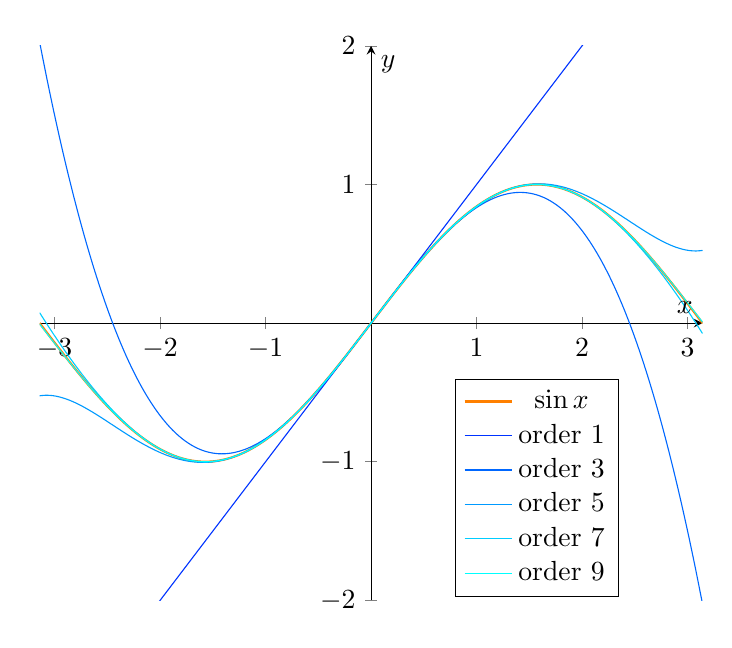
\begin{tikzpicture}
        \begin{axis}[width=10cm,domain=-pi:pi,samples=101,smooth,
        no markers,axis lines=middle,
        legend style={at={(0.75,0.4)},anchor=north},
        ymax=2,ymin=-2,xlabel=$x$,ylabel=$y$,
        colormap={blueblack}{color=(blue) color=(cyan)},
        cycle multiindex* list={[samples of colormap=6]\nextlist mark list\nextlist}]
            \addplot[thick,color=orange,domain=-pi:pi] {sin(deg(x))};
            \addlegendentry{$\sin x$}
            \edef\myfun{0}
            \pgfplotsforeachungrouped \nn in {0,1,2,3,4}
            {\edef\myfun{\myfun+((-1)^(\nn))*pow(x,2*\nn+1)/factorial(2*\nn+1)}
             \addplot+{\myfun};
             \addlegendentryexpanded{order $\the\numexpr2*\nn+1$}
            }
        \end{axis}
    \end{tikzpicture}
    \caption{The plot of the original function is barely visible because we have a pretty good approximation using just polynomials.}
    \label{fig:sine_maclaurin}
\end{figure}

For our purposes, being able to identify patterns in infinite series that
suggest they are approximations for other, more well-known functions is
sufficient. See \cref{tab:common_maclaurin} below for some of the more common
examples (for $x_{0}=0$) that will show up in the upcoming lessons.

\begin{table}[ht]
    \centering
    \sffamily
    \begin{tabular}{ccc}
         \toprule
         \textbf{Function} & \textbf{Maclaurin Series} & \textbf{Interval of Convergence} \\
         \midrule
         $\displaystyle \frac{1}{1-x}$ & $\displaystyle \sum_{n=0}^{\infty} x^{n}$  & $-1 < x < 1$ \\ [1.6em]
         $\displaystyle e^{x}$ & $\displaystyle \sum_{n=0}^{\infty} \frac{x^{n}}{n!}$  & $-\infty < x < \infty$ \\ [1.6em]
         $\displaystyle \ln(1+x)$ & $\displaystyle \sum_{n=1}^{\infty} \frac{(-1)^{n+1}x^{n}}{n}$  & $-1 < x \leq 1$ \\ [1.6em]
         $\displaystyle \sin(x)$ & $\displaystyle \sum_{n=0}^{\infty} \frac{(-1)^{n+1}x^{2n+1}}{(2n+1)!}$ & $-\infty < x < \infty$ \\ [1.6em]
         $\displaystyle \cos(x)$ & $\displaystyle \sum_{n=0}^{\infty} \frac{(-1)^{n}x^{2n}}{(2n)!}$ & $-\infty < x < \infty$ \\
         \bottomrule
    \end{tabular}
    \caption{The interval of convergence governs where this approximation works.}
    \label{tab:common_maclaurin}
\end{table}

\end{document}
